% Unofficial University of Cambridge Poster Template
% https://github.com/andiac/gemini-cam
% a fork of https://github.com/anishathalye/gemini
% also refer to https://github.com/k4rtik/uchicago-poster

\documentclass[final]{beamer}

% ====================
% Packages
% ====================

\usepackage[T1]{fontenc}
\usepackage{lmodern}
\usepackage[orientation=portrait,size=a0,scale=1.25]{beamerposter}
\usetheme{gemini}
\usecolortheme{nott}
\usepackage{graphicx}
\usepackage{booktabs}
\usepackage{tikz}
\usepackage{pgfplots}
\pgfplotsset{compat=1.14}
\usepackage{anyfontsize}


% for tables
\usepackage{multirow}
\usepackage{multicol}
\usepackage{transparent}

% for urls
\usepackage{hyperref}

% for subfigures
\usepackage{caption}
\usepackage{subcaption}

% for bibliography
\renewcommand{\refname}{Literature}
\usepackage[backend=biber]{biblatex}
\addbibresource{../presentation/references.bib}

% for inline code listings
\usepackage{listings}
\usepackage{xparse}
\usepackage{xcolor}
\definecolor{codeblue}{rgb}{0.0, 0.0, 1.0}
\definecolor{codegreen}{rgb}{0.0, 0.5, 0.0}
\definecolor{codegray}{rgb}{0.5, 0.5, 0.5}
\definecolor{codepurple}{rgb}{0.58, 0.0, 0.82}
\definecolor{backcolour}{rgb}{0.95, 0.95, 0.92}
\lstdefinestyle{py}{
    language=Python,
    %  backgroundcolor=\color{backcolour},
    commentstyle=\color{codegreen},
    keywordstyle=\color{codeblue},
    numberstyle=\tiny\color{codegray},
    stringstyle=\color{codepurple},
    basicstyle=\small\ttfamily,
    breakatwhitespace=false,
    breaklines=true,
    captionpos=b,
    keepspaces=true,
    numbers=left,
    numbersep=5pt,
    showspaces=false,
    showstringspaces=false,
    showtabs=false,
    tabsize=4,
    frame=0,
    rulecolor=\color{black},
    morekeywords={self, assert, yield, None, True, False}
}

% ====================
% Lengths
% ====================

% If you have N columns, choose \sepwidth and \colwidth such that
% (N+1)*\sepwidth + N*\colwidth = \paperwidth
\newlength{\sepwidth}
\newlength{\colwidth}
\setlength{\sepwidth}{0.025\paperwidth}
\setlength{\colwidth}{0.45\paperwidth}

\newcommand{\separatorcolumn}{\begin{column}{\sepwidth}\end{column}}

% ====================
% Title
% ====================

% Title page
\title{\Large Network Diffusion --- Framework to Simulate Spreading Processes in Complex Networks}
\author{\large
    \textbf{Micha{\l} Czuba} \inst{1},
    Mateusz Nurek \inst{1},
    Damian Serwata \inst{1},
    Yu-Xuan Qi \inst{2},
    Mingshan Jia \inst{2},
    Katarzyna Musial \inst{2},
    Rados{\l}aw Michalski \inst{1},
    Piotr Br{\'o}dka \inst{1}
}
\institute{
  \inst{1} Wroc{\l}aw University of Science and Technology\\
  \inst{2} University of Technology Sydney
}

% ====================
% Footer (optional)
% ====================

\footercontent{
  \href{https://networks.pwr.edu.pl/}{https://networks.pwr.edu.pl} \hfill
  NetSci, Canada, July 2023 \hfill
  \href{mailto:michal.czuba@pwr.edu.pl}{michal.czuba@pwr.edu.pl}}

% ====================
% Logo (optional)
% ====================

\logoright{
\includegraphics[height=4cm]{logos/nsl-white.pdf}}
\logoleft{
\includegraphics[height=4cm]{logos/wust_logo.pdf}}

% ====================
% Body
% ====================

\begin{document}

\begin{frame}[t, fragile]
\begin{columns}[t]

\separatorcolumn
\begin{column}{\colwidth}

\begin{block}{Introduction}
    Spreading phenomena are one of the issues considered by a network science. They can be obeserved
    in various areas like: dynamics of political opinions, marketing campaigns, spread of epidemics,
    computer viruses, etc. With the advancement of computational network science analytical 
    approaches became insufficient for large graphs, prompting researchers to use computational
    methods. In recent years, the scope of network science has significantly expanded beyond static
    graphs to encompass more complex structures. The introduction of streaming, temporal, multilayer,
    and hypernetwork approaches has brought new possibilities and imposed additional requirements.
    Unfortunately, the pace of advancement is often too rapid for existing computational packages to
    keep up with the functionality updates...
\end{block}

\begin{alertblock}{Problem}
    There is a bunch of very good and robust tools that helps in sumulating diffusion processes in 
    networks, e.g. \lstinline[style=py]{ndlib} (which we love). \\
    \vspace{2em}
    However, if we consider...\\
    \vspace{1em}
    \hspace{5em}...more complex network models,... \\
    \vspace{1em}
    \hspace{5em}...spreading multiple processes at the same time... \\
    \vspace{1em}
    \hspace{14em}...\textbf{a gap among the available toolkits} emerges.
\end{alertblock}

\begin{block}{Our Contribution}
    In order to address the issue, we decided to redesign, polish, and share our internal 
    environment which we are using in the lab. Thus, in our recent work~\cite{czuba2024networkdiffusion},
    we presented \lstinline[style=py]{network-diffusion}. To start using the library just type in 
    your shell:
    \begin{center}
        \large
        \begin{verbatim}
            pip install network-diffusion
        \end{verbatim}
    \end{center}
    \vspace{-1em}
    Or scan this code to reach the docs with more examples:
    \begin{figure}
        
\includegraphics[width=15cm]{../presentation/figures/qr_code.pdf}
    \end{figure}
\end{block}

\begin{block}{Key Features}
    \begin{itemize}
        \item \textbf{End-to-End Simulation Workflow}: The library enables users 
        to simulate diffusion processes in complex networks with ease. Whether
        you are studying information spread, disease propagation, or any other
        diffusion phenomena, this library has you covered.
        \item \textbf{Support for Temporal Network Models}: You can work with temporal models, allowing you to
        capture the dynamics of processes over time. These temporal models can be
        created using regular time windows or leverage \textbf{CogSnet}.
        \item \textbf{Support for Multilayer Network Models}: The library supports multilayer networks, which are
        essential for modelling real-world systems with interconnected layers of
        complexity
        \item \textbf{Predefined Spreading Models}: You have the option to use predefined diffusion 
        models such as the Linear Threshold Model, Independent Cascade Model, and more. Those are
        implemented to simplify the simulation process, allowing users to focus on their specific
        research questions.
        \item \textbf{An Interface for Implementing Custom Spreading Models}: Additionally, 
        \lstinline[style=py]{network-diffusion} allows you to define your own diffusion models using
        open interfaces, providing flexibility for researchers to tailor simulations to their unique
        requirements.
        \item \textbf{New Centrality Measures}: The library provides a wide range of centrality 
        measures specifically designed for multilayer networks. These measures can be valuable for
        selecting influential seed nodes in diffusion processes.
        \item \textbf{NetworkX Compatibility}: The package is built on top of  
        \lstinline[style=py]{networkx}, ensuring seamless compatibility with this popular Python 
        library for network analysis. You can easily integrate it into your existing
        \lstinline[style=py]{networkx}-based workflows.
    \end{itemize}
\end{block}

\end{column}

\separatorcolumn
\begin{column}{\colwidth}

\begin{alertblock}{Example}

    \heading{Extending Linear Threshold Model to multilayer Networks}
    In a diffusion under Linear Threshold Model~\cite{kempe2003maximizing}, each node:
    \begin{itemize}
        \item can fall in two states: \textit{active} and \textit{inactive},
        \item becomes \textit{active} if the fraction of its \textit{active} neighbors to all 
        neighbours exceeds certain threshold ($\mu$).
    \end{itemize}
    In case of multilayer networks --- \textbf{actors are the subject of the process, while the 
    nodes are their auxiliary representation}. Thus, we have to define how to aggregate impulses 
    from the layers. In this example we will consider method introduced by~\cite{zhong2022mltm} --- 
    a protocol functions, namely "OR" variant which says that the actor can be activated if any of 
    nodes representing it gets activated.

    \heading{Visualisation}
    \begin{figure}
        \centering
        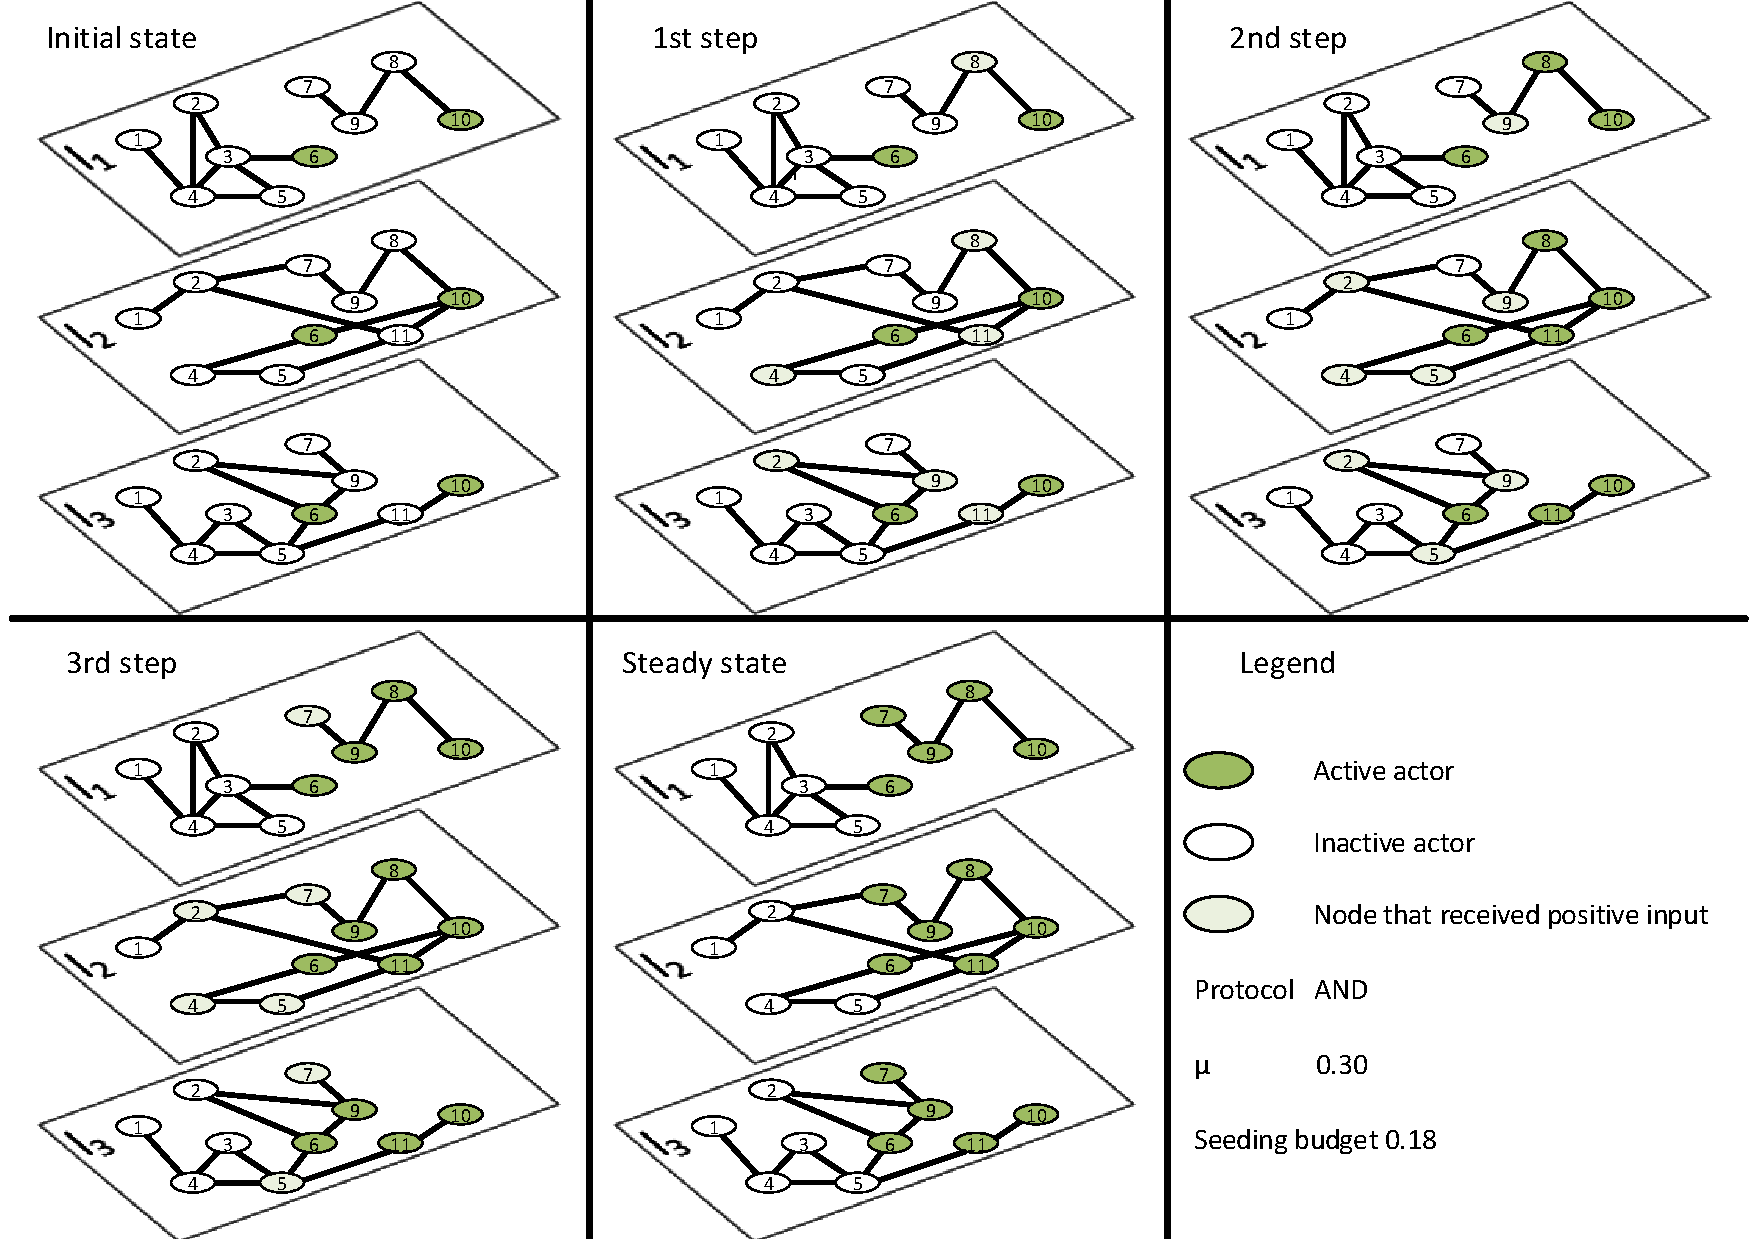
\includegraphics[width=1\linewidth]{figures/ltm_example.pdf}
        \caption{Example of spreading of MLTM in toy network with protocol $AND$.}
        \label{fig:ltm_example_and}
    \end{figure}
% \end{alertblock}

% \begin{alertblock}{A Short Example}


% \begin{block}{Linear Threshold Model}
%     Each node:
%     \begin{itemize}
%         \item can fall in two states: \textit{active} and \textit{inactive},
%         \item becomes \textit{active} if the fraction of its \textit{active} neighbors to all neighbours
%         exceeds certain threshold.
%     \end{itemize}
%     \end{block}
%     In case of multilayer networks the actors not the nodes\footnote{which can be considered as avatars
%     of the actors on the network's layers} are a subject of the diffusion. Thus, we have to define
%     how to aggregate impulses from the layers. In this example we will consider "OR" strategy, which 
%     says that the actor can be activated if any of nodes representing it in the network gets activated.

%     \begin{figure}
%         \centering
%         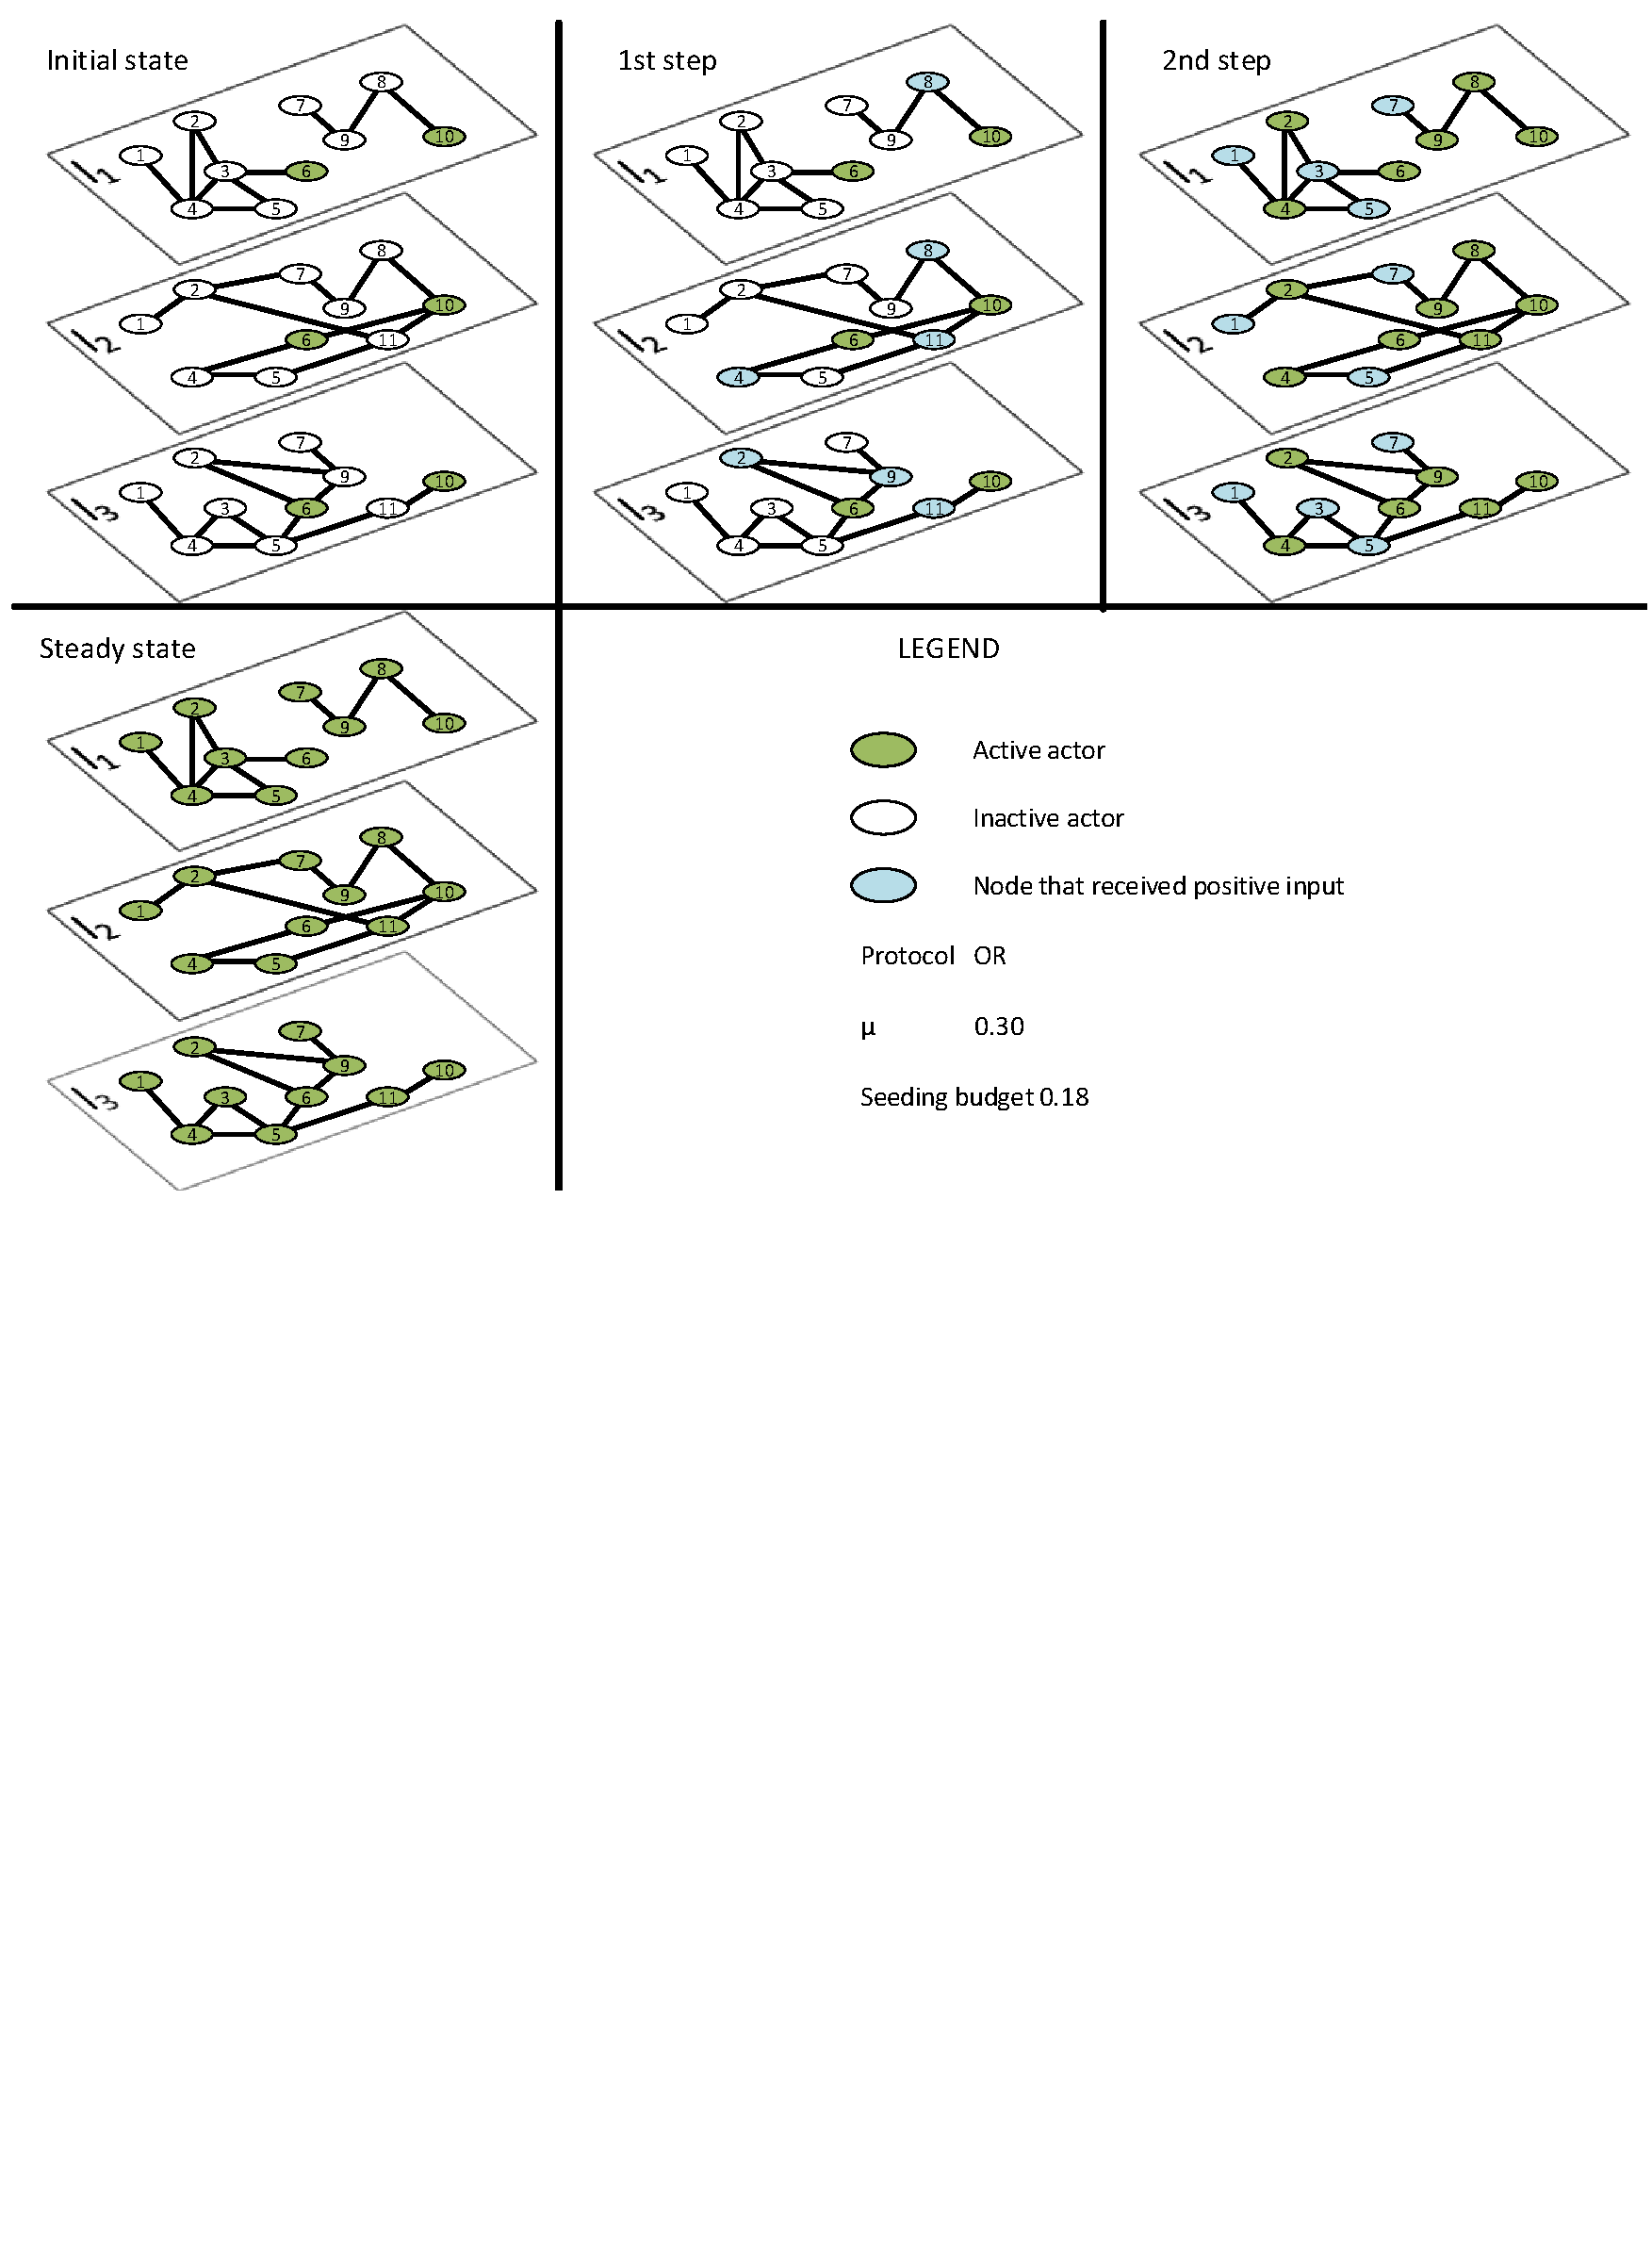
\includegraphics[width=.75\textwidth]{../presentation/figures/ltm_example_or.pdf}
%         \caption{Propagation according to LTM with the $OR$ strategy in a multilayer network -
%         active actors: seeds $\{6, 10\}$, in a stable state: all of them.}
%     \end{figure}

\heading{Modelling this case with \lstinline[style=py, basicstyle=\large\ttfamily]{network-diffusion}}

\begin{lstlisting}[style=py, basicstyle=\footnotesize\ttfamily]
import network_diffusion as nd

# define the model with its internal parameters
spreading_model = nd.models.MICModel(
    seeding_budget=[90, 10, 0],  # 95% act suspected, 10% infected, 0% recovered
    seed_selector=nd.seeding.RandomSeedSelector(),  # pick infected act randomly
    protocol="OR",  # how to aggregate impulses from the network's layers
    probability=0.5,  # probability of infection
)

# get the graph - a medium for spreading
network = nd.mln.functions.get_toy_network_piotr()

# perform the simulation that lasts four epochs
simulator = nd.Simulator(model=spreading_model, network=network)
logs = simulator.perform_propagation(n_epochs=3)

# obtain detailed logs for each actor in the form of JSON
raw_logs_json = logs.get_detailed_logs()

# or obtain aggregated logs for each of the network's layer
aggregated_logs_json = logs.get_aggragated_logs()

# or just save a summary of the experiment with all the experiment's details
logs.report(visualisation=True, path="my_experiment")
\end{lstlisting}

\heading{Outcomes}

% 6. Save experiment results. User is able to save them to the file or print them out

% .. literalinclude:: simulator_example.py
%    :language: python
%    :lines: 249

% The logs contain:
% * a description of the network (txt file),
% * a description of the propagation model (txt file),
% * a report of the spreading for all simulated phenomena (separate csv files),
% * a capture of states of every single node at the end of each simulation step (JSON file),
% * a brief visualisation of propagation.

% .. figure:: images/experiment_vis.png
%     :width: 600

% In case of need to process the results directly in the Python, one can extract them with two
% functions. For aggregated results for each process

% .. literalinclude:: simulator_example.py
%    :language: python
%    :lines: 253

% or for the detailed logs concerning all nodes

% .. literalinclude:: simulator_example.py
%    :language: python
%    :lines: 257


\end{alertblock}

\begin{block}{References}
    \printbibliography
\end{block}

\end{column}
\separatorcolumn

\end{columns}
\end{frame}

\end{document}
